\section{Experiments and Analysis}
\label{sec:experiments}
\accuracyTable
\textbf{Baselines.} 
We compare \sysname against two groups of methods. (1) Three state-of-the-art SVD-based LLM compression methods: FWSVD~\citep{DBLP:conf/iclr/HsuHCLSJ22}, ASVD~\citep{DBLP:journals/corr/abs-2312-05821}, and SVD-LLM~\citep{DBLP:journals/corr/abs-2403-07378} (Section~\ref{subsec:overall_performance}). (2) Other types of LLM compression methods. These include three state-of-the-art pruning-based LLM compression methods: LLM-Pruner~\citep{DBLP:conf/nips/MaFW23}, SliceGPT~\citep{DBLP:conf/iclr/AshkboosCNHH24}, and BlockPruner~\citep{DBLP:journals/corr/abs-2406-10594}, and two state-of-the-art quantization-based LLM compression methods: PB-LLM~\citep{DBLP:conf/iclr/YuanSD24}, and BiLLM~\citep{DBLP:conf/icml/HuangLQLZ0M024} (Section~\ref{subsection:Comparison_with_other_compression_methods}).

\vspace{1mm}
\noindent\textbf{Models and Datasets.} To demonstrate the generability of our method, we evaluate the performance of \sysname on five models at various scales (LLaMA-7B, 13B, 30B, LLaMA3-8B~\citep{DBLP:journals/corr/abs-2307-09288}, OPT-6.7B~\citep{DBLP:journals/corr/abs-2205-01068}) and ten datasets including two language modeling datasets (WikiText-2~\citep{DBLP:conf/iclr/MerityX0S17} and C4~\citep{DBLP:journals/jmlr/RaffelSRLNMZLL20}), six classification datasets (OpenbookQA~\citep{DBLP:conf/emnlp/MihaylovCKS18}, WinoGrande~\citep{DBLP:conf/aaai/SakaguchiBBC20}, HellaSwag~\citep{DBLP:conf/acl/ZellersHBFC19}, Arc\_e~\citep{DBLP:journals/corr/abs-1803-05457}, PIQA~\citep{DBLP:conf/aaai/BiskZLGC20}, MathQA~\citep{DBLP:conf/naacl/AminiGLKCH19}),  and two generation datasets (TruthfulQA~\citep{DBLP:conf/acl/LinHE22} and GSM8K~\citep{DBLP:journals/corr/abs-2110-14168})  with the LM-Evaluation-Harness framework~\citep{eval-harness}.

\vspace{1mm}
\noindent\textbf{Implementation Details.} 
We randomly select $256$ WikiText-2 samples as the calibration data. To mitigate the error raised by the Choleksy decomposition in SVD-LLM due to positive definite, we followed the implementation of SVD-LLM~\citep{DBLP:journals/corr/abs-2403-07378} to add the small noise into the decomposed matrices. The compression ration in our experiments refers to the parameter reduction of LLM achieved through compression. All of the experiments are conducted on A100 GPUs.

\subsection{Performance Comparison}
\label{subsec:overall_performance}
%To examine the generability of \sysname, 
We first compare \sysname against state-of-the-art SVD-based LLM compression methods from four aspects: (1) performance on different LLMs, (2) performance on LLMs with larger scales, (3) performance under different compression ratios, and (4) compression speed.

\vspace{1mm}
\noindent\textbf{Performance on Different LLMs.} 
We compare the performance between \sysname and the baselines on three different LLMs, including LLaMA-7B, OPT-6.7B, and LLaMA-3 8B  under 20\% compression ratio on ten datasets. As shown in~\cref{tab:dataset_acc},  \sysname consistently achieves better and more stable performance than all the SVD-based LLM compression baselines across all three LLMs and all ten datasets. 
%
In particular, \sysname achieves up tp 42\% perplexity reduction and 9\% accuracy
improvement with better generation ability compared to prior state-of-the-art method SVD-LLM on LLaMA-3 8B.

\vspace{1mm}
\noindent\textbf{Performance on LLMs with Larger Scales.} 
We compare the performance between \sysname and the baselines on LLaMA-13B and LLaMA-30B under 20\% compression ratio on WikiText-2 and six classification datasets. As shown in~\cref{tab:large_llm_acc}, \sysname consistently outperforms all the baselines on both 13B and 30B model sizes. 


\largellmaccuracyTable

\vspace{1mm}
\noindent\textbf{Performance under Different Compression Ratios.}
We compare the performance between \sysname and the baselines on LLaMA-7B under compression ratio ranging from 20\% to 80\% on WikiText-2 and six classification datasets. As shown in~\cref{fig:ratio}, \sysname consistently outperforms all baselines, and the performance gain compared to the best-performing baseline increases as the compression ratio increases. 

\vspace{1mm}
\noindent\textbf{Compression Speed.}
Besides measuring the performance of the compressed LLMs, we also evaluate the compression speed. Specifically, we measure the A100 GPU hours used by \sysname and the baseline methods for compressing LLaMA-7B under 20\% compression ratio. 
%
Our results show that FWSVD takes about 6 GPU hours, ASVD takes about 5.5 GPU hours, SVD-LLM takes about 15 minutes, and \sysname takes about 18 minutes to finish the compression. 
%
FWSVD requires gradient calculation, thus consumes a significant amount of time for compression. 
%
For the other methods, the main reason for such a variation is their respective techniques for allocating compression ratios among weight matrices. SVD-LLM assigns the same compression ratio to all weight matrices, enabling the fastest operation but sacrificing accuracy. ASVD, however, determines the compression ratio by regularly evaluating the end-to-end perplexity, which slows down its compression process. In contrast, \sysname allocates the compression ratio directly from its truncation loss, making it significantly faster than ASVD.


\begin{figure}[t]
    \begin{subfigure}{0.48\textwidth}
            \centering
            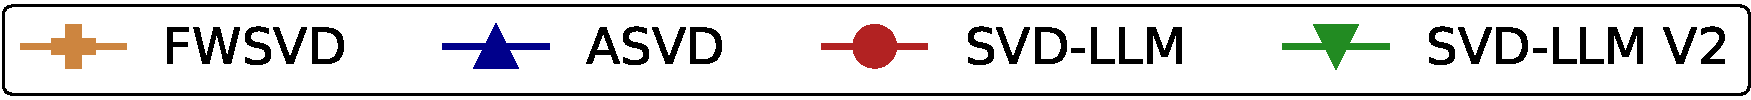
\includegraphics[width=\linewidth]{Figures/ratio_legend.pdf}
            % \vspace{1mm}
        \end{subfigure}
        \\
         \begin{subfigure}{0.235\textwidth}
            \centering
            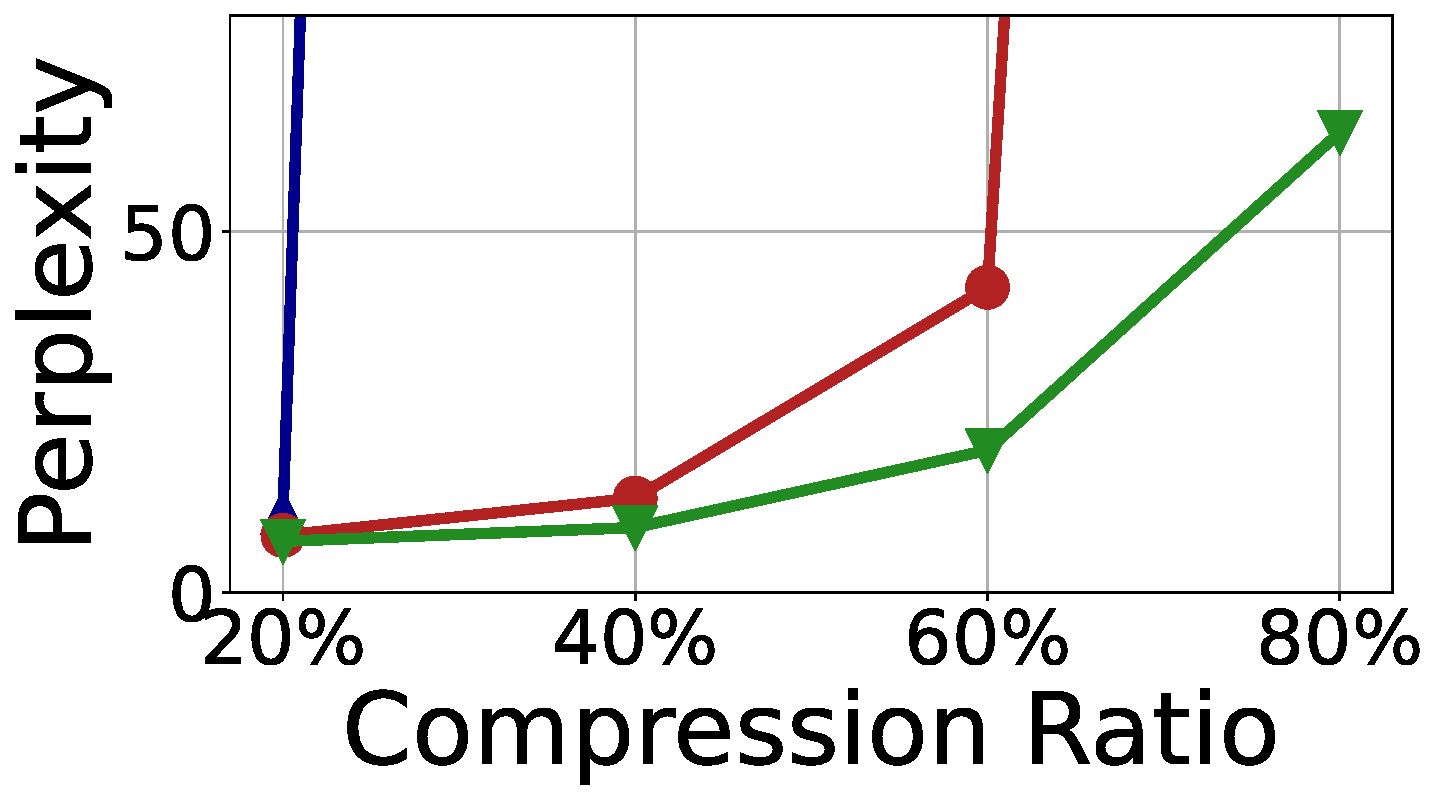
\includegraphics[width=\linewidth]{Figures/ppl_ratio.pdf}  % 插入图像
            \caption{Perplexity}
            \label{fig:ppl_ratio}
        \end{subfigure}
        \begin{subfigure}{0.235\textwidth}
            \centering
            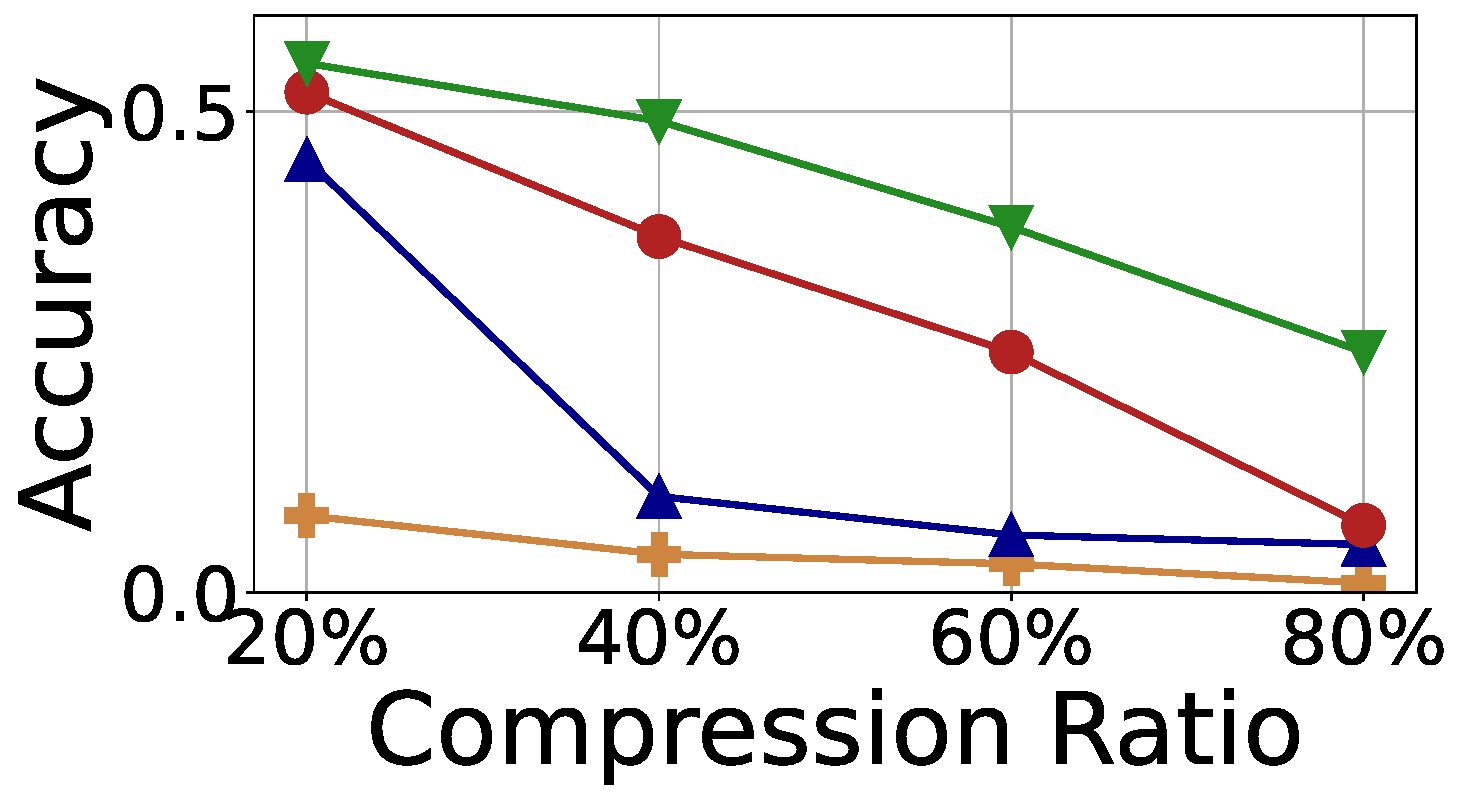
\includegraphics[width=\linewidth]{Figures/acc_ratio.pdf}  % 插入图像
            \caption{Average Accuracy}
            \label{fig:acc_ratio}
        \end{subfigure}
\caption{Perplexity on WikiText-2 and average accuracy on six classification datasets of LLaMA-7B compressed by \sysname  and other SVD-based LLM compression baselines under 20\% to 80\% compression ratios. The perplexity values of FWSVD and ASVD are larger than 100, thus are not shown in the figure.}
\vspace{-5mm}
\label{fig:ratio}
\end{figure}

\subsection{Inference Speedup of \sysname }
\label{subsec:inference_speedup}
% \vspace{-2mm}
To evaluate the inference speedup of models compressed by \sysname, we measure the numbers of tokens generated per second from both the original LLaMA-7B and the model compressed by \sysname under different compression ratios on a single NVIDIA A100 GPU. 
%
For a fair comparison, we fix the batch size to 4, the prefill length to 1024,  and the decoding length to 256. As shown in~\cref{fig:speedup}, \sysname consistently achieves faster token generation speeds across all the compression ratios. 
%
More importantly, the speedup becomes more significant as the compression ratio increases, resulting in a speedup of 1.29x under 20\% compression ratio, 1.63x under 40\% compression ratio, 2.08x under 60\% compression ratio, and 2.71x under 80\% compression ratio. 

% \vspace{-2mm}
\begin{figure}[t]
    \centering
    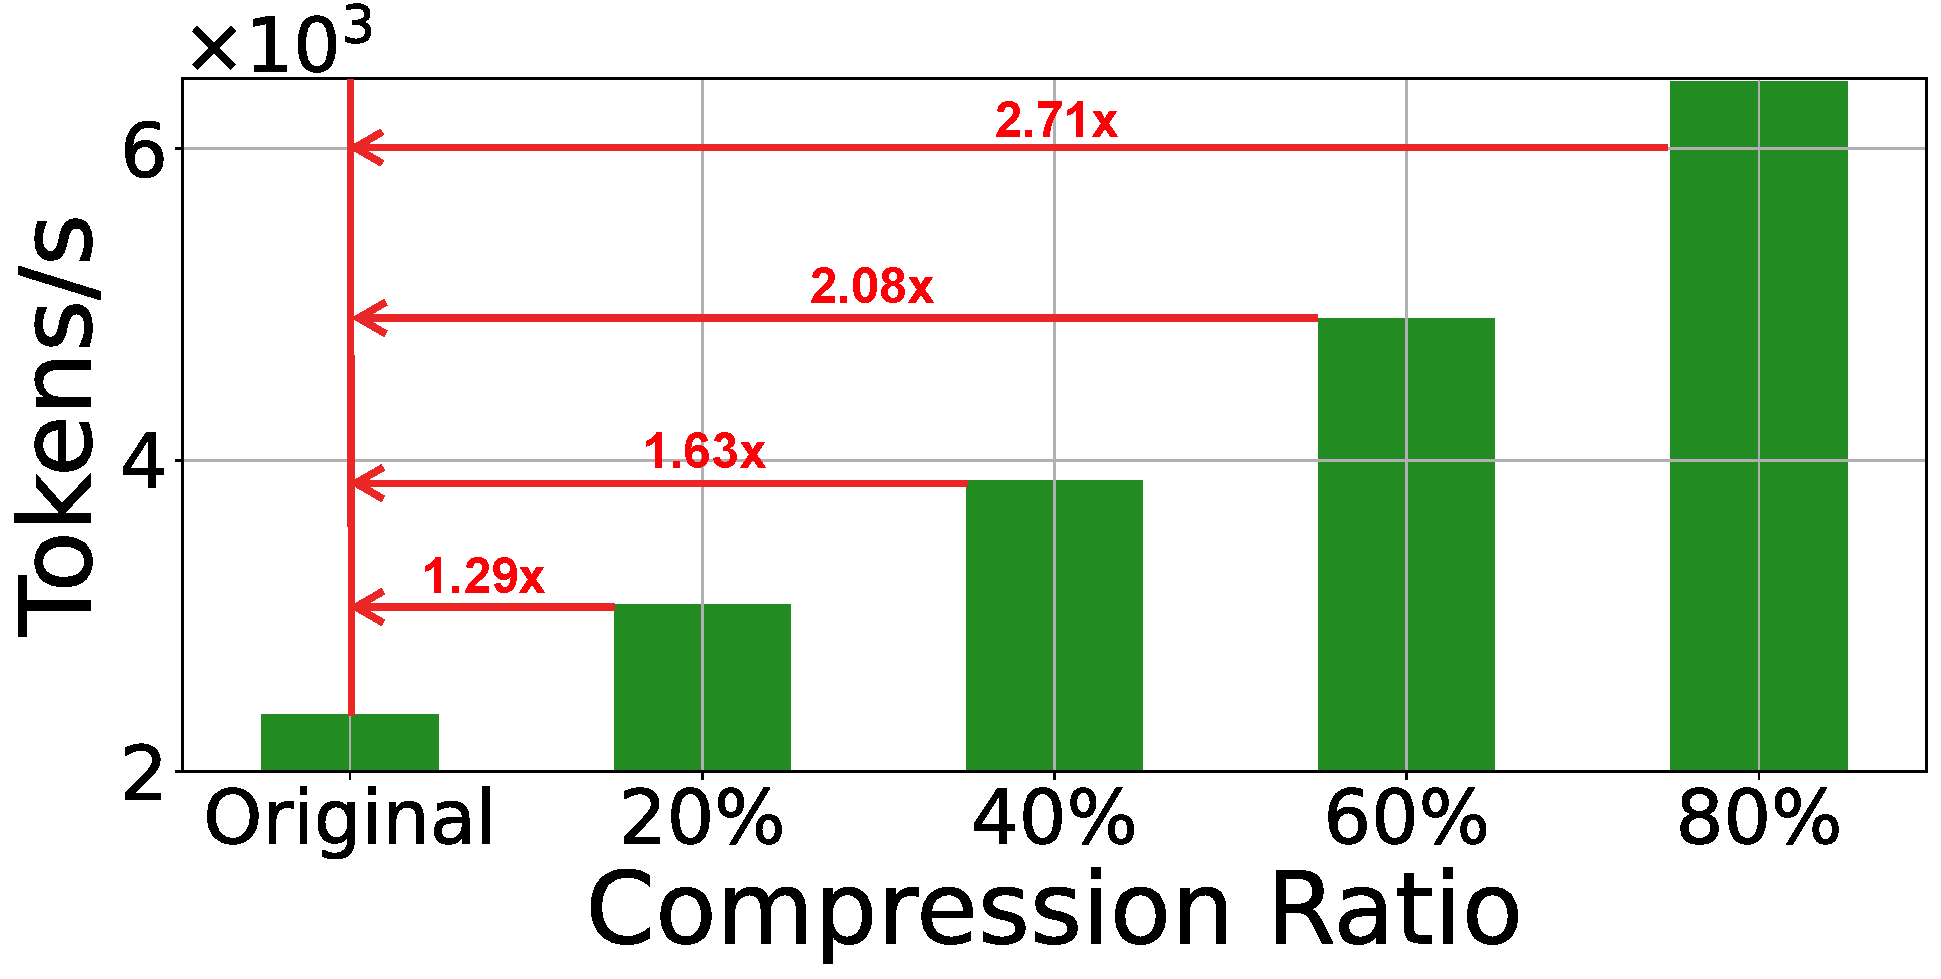
\includegraphics[width=0.4\textwidth]{Figures/Speedup.pdf}
    \caption{Throughput (Tokens/s) achieved by original LLaMA-7B and its compressed version by \sysname under different compression ratios on a single NVIDIA A100 GPU. We fix the batch size to 4, prefill length to 1024,  and decoding length to 256.  The speedup over the original LLM is marked in red.}
    \label{fig:speedup}
    % \vspace{-10mm}
\end{figure}

\vspace{2mm}
\sensitivityTable

\subsection{Ablation Study}
\label{subsec:ablation_study}
\sysname has two key components, both of which optimize the truncation loss. 
%
In our ablation study, we first evaluate the individual contribution of each of the two components to the compression performance. 
%
Next, since both components fully utilize the whitening matrix $S$, which is calculated with a randomly selected calibration set, we evaluate the impacts of different calibration data on the performance of \sysname.

\vspace{1mm}
\noindent\textbf{Component Sensitivity Study.} We first evaluate the individual contribution of the two components (i.e., heterogeneous compression ratio allocation and loss-optimized weight truncation) of \sysname. 
%
Let \sysname (A) denote the version of \sysname with heterogeneous compression ratio allocation only; and \sysname (T) denote the version of \sysname with loss-optimized weight truncation only.
%; and \sysname (A+T) denote the version of \sysname with both heterogeneous compression ratio allocation and loss-optimized weight truncation.
%
The results are shown in~\cref{tab:sensitivity}. We have two observations. 
%
(1) Both \sysname (A) and \sysname (T) outperform SVD-LLM, demonstrating the effectiveness of each of these two components alone in achieving superior compression performance.
%
(2) \sysname outperforms \sysname (A) and \sysname (T), demonstrating the necessity of having both components.

\vspace{1mm}
\noindent\textbf{Impact of Calibration Set.} Next, we examine the impact of the calibration set on the compression performance of \sysname. Specifically, we measure the changes in perplexity of LLaMA-7B compressed by \sysname under 20\% compression ratio on WikiText-2 when using the default calibration set but with various numbers of data and sampling seeds.
%
As shown in~\cref{fig:calibration}, the changes in both data number and sampling seed in the calibration set incur no more than 1\% fluctuation in the final performance, demonstrating that \sysname is not sensitive to the calibration set.

\begin{figure}[t]
         \begin{subfigure}{0.235\textwidth}
            \centering
            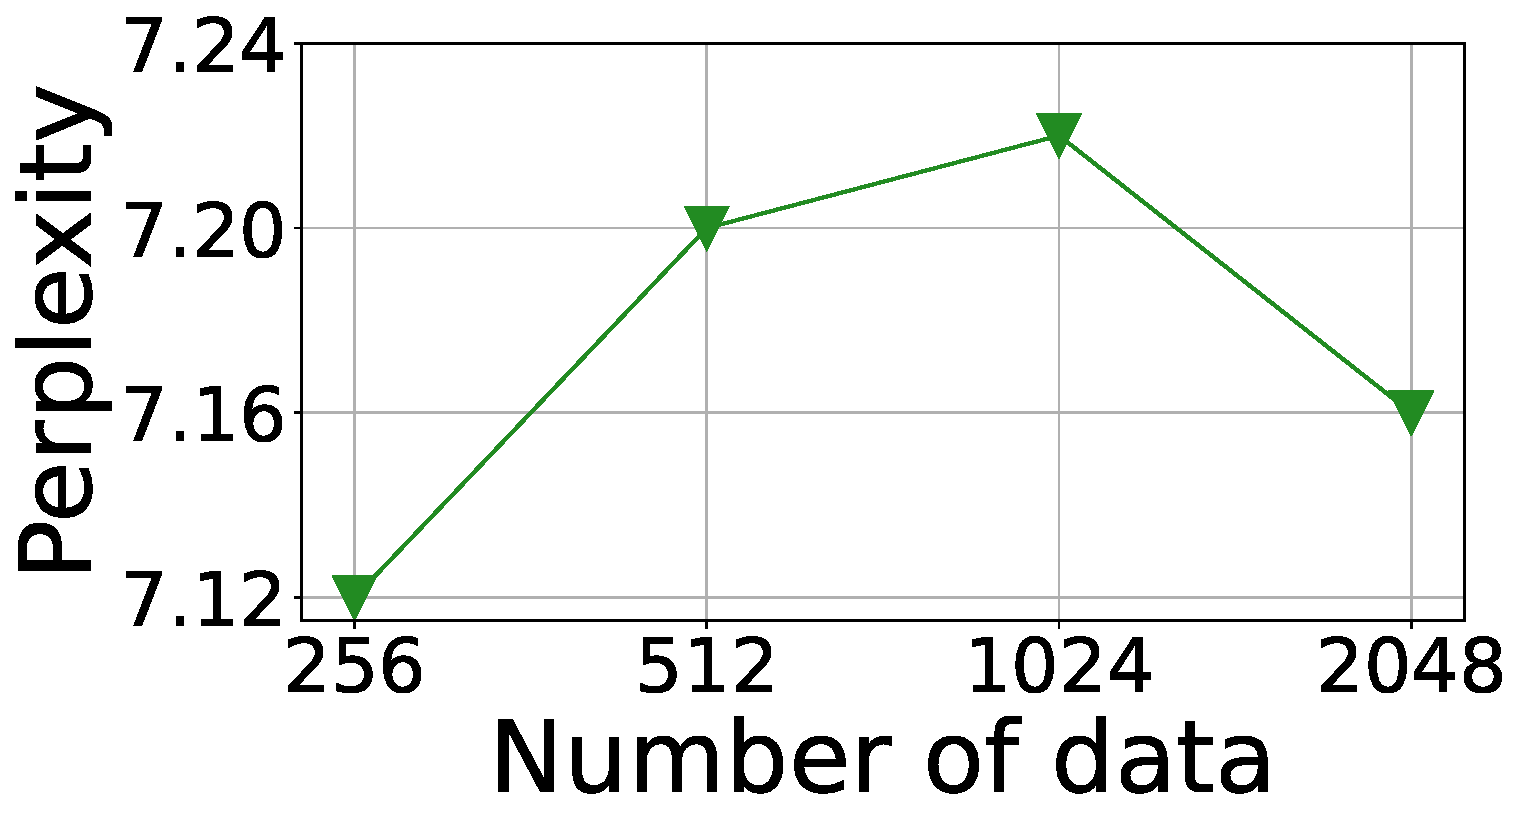
\includegraphics[width=\linewidth]{Figures/cali_size.pdf}  % 插入图像
            \caption{Various Data Number}
            \label{fig:cali_number}
        \end{subfigure}
        \begin{subfigure}{0.24\textwidth}
            \centering
            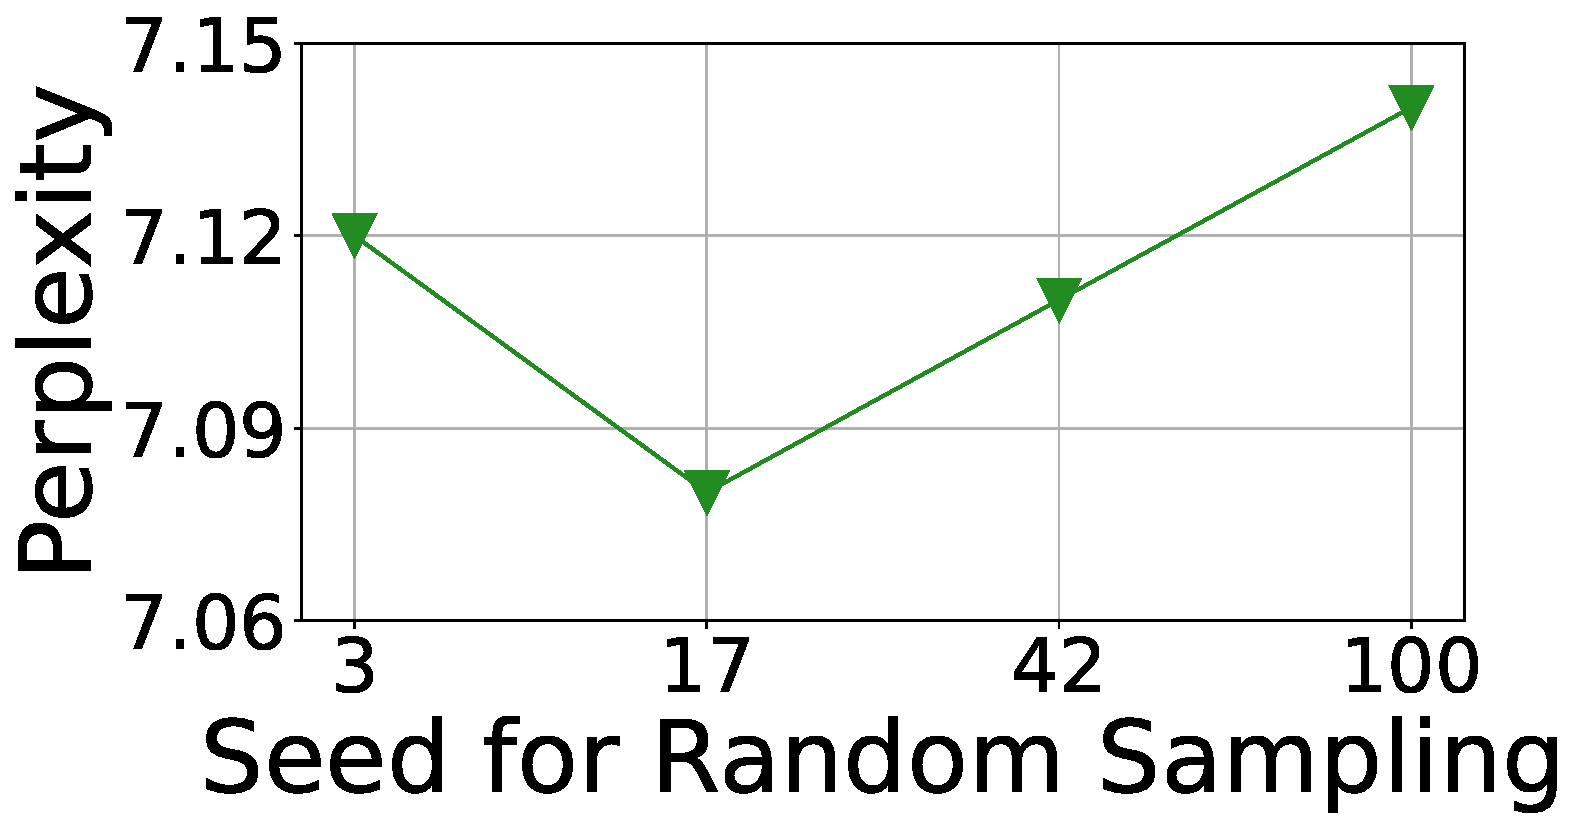
\includegraphics[width=\linewidth]{Figures/seed.pdf}  % 插入图像
            \caption{Various Samping Seed}
            \label{fig:cali_seed}
        \end{subfigure}
\caption{Perplexity of LLaMA-7B under 20\% compression ratio using calibration data sampled with different numbers or seeds from WikiText-2.}
\label{fig:calibration}
\end{figure}

\subsection{Comparison with Other Types of Post-training LLM Compression Methods} 
\sysname is orthogonal to other post-training LLM compression methods, including quantization and pruning. In this experiment, we compare the performance of \sysname with state-of-the-art structured pruning-based and quantization-based LLM compression methods. 

\svdprunepplTable

% \vspace{-8mm}
\svdpruneaccTable

\noindent\textbf{Comparison with Structured Pruning.}
First, we compare \sysname with three state-of-the-art post-training structured pruning-based LLM compression methods: LLM-Pruner~\citep{DBLP:conf/nips/MaFW23}, SliceGPT~\citep{DBLP:conf/iclr/AshkboosCNHH24}, and BlockPruner~\citep{DBLP:journals/corr/abs-2406-10594} under various weight memory budgets, ranging from 10 GB to 7 GB. 
%
The perplexity results are shown in~\cref{tab:svd_prune_ppl} and the average accuracy results are shown in~\cref{tab:svd_prune_acc}. 
%
As shown, \sysname outperforms all three state-of-the-art structured pruning-based LLM compression methods. In particular, under 7 GB memory budget, \sysname achieves 28\% reduction in perplexity and 13\% higher average accuracy.


\vspace{1mm}
\noindent\textbf{Comparison with Quantization.} 
%
Next, we compare \sysname with post-training quantization-based LLM compression methods. 
%
We first compare \sysname with GPTQ~\citep{DBLP:journals/corr/abs-2210-17323} under 3-bit quantization. As shown in~\cref{tab:svd_quant_4bit}, while \sysname achieves worse perplexity compared to GPTQ under 3-bit memory budget, 
%it still remains highly useful for moderate compression ratios. 
%This is because 
combining \sysname (30\% compression ratio) with GPTQ-4-bit achieves superior perplexity compared to GPTQ-3-bit under the same memory budget. 
%Specifically, because SVD-based compression is orthogonal to and can be seamlessly combined with quantization-based methods, 
In other words, we find that under the same memory budget, by first compressing the original 16-bit LLM with \sysname at 30\% compression ratio, then quantizing the compressed LLM to 4-bit using GPTQ, we are able to achieve better perplexity compared to directly quantizing the original LLM to 3-bit.  
%
Finally, we compare \sysname with  two state-of-the-art post-training quantization-based LLM compression methods: BiLLM~\citep{DBLP:conf/icml/HuangLQLZ0M024} and PB-LLM~\citep{DBLP:conf/iclr/YuanSD24}, which push the frontier to 1-bit quantization.
%under 1-bit quantization. 
%
The results are shown in Table~\ref{tab:svd_quant}. 
%
We have two observations: (1) Without combining with quantization techniques, \sysname (16-bit) outperforms PB-LLM with 5\% lower perplexity.
%
%achieves a performance comparable to several 1-bit post-training quantization methods. In particular, it achieves 5\% lower perplexity than PB-LLM~\citep{DBLP:conf/iclr/YuanSD24}, highlighting the effectiveness of \sysname in compressing LLM to the extremely low memory budge similar to 1-bit quantization. 
%
(2) By combining with quantization techniques, \sysname (2-bit) outperforms state-of-the-art 1-bit post-training quantization method BiLLM. In particular, \sysname (2-bit) achieves 69\% lower perplexity than BiLLM, showing the promise of combining SVD-based and quantization-based compression methods for pushing the frontier of post-training LLM compression forward.
%a new research avenue that combines \sysname with recent quantization methods to further enhance compression performance.


\vspace{0mm}
\svdquanthighTable

\vspace{0mm}
\svdquantTable

\label{subsection:Comparison_with_other_compression_methods}